\begin{frame}[hasprev=false, hasnext=true]
\label{example:tacoma-narrows-bridge}
\frametitle{Tacoma Narrows Bridge}
\framesubtitle{Description}

\begin{itemize}
	\item The Tacoma Narrows Bridge is a pair of mile-long suspension bridges
	in the U.S. state of Washington, across the Tacoma Narrows, between Tacoma
	and the Kitsap Peninsula.

	\item It was opened to traffic on July 1, 1940.
\end{itemize}

\begin{figure}
	\centering
	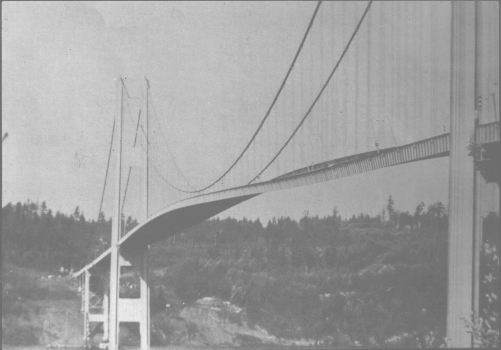
\includegraphics[width=.5\textwidth]{aux/examples/tacoma-narrows-bridge/tacoma-narrows-bridge}
\end{figure}
\end{frame}



\begin{frame}[hasprev=true, hasnext=true]
\frametitle{Tacoma Narrows Bridge}
\framesubtitle{Problem}

\begin{itemize}
	\item It collapsed four months later on November 7, 1940, at 11:00 AM
	(Pacific time) due to a physical phenomenon known as aeroelastic flutter
	caused by a 67 kilometers per hour (42 mph) wind.
\end{itemize}

\begin{figure}
	\centering
	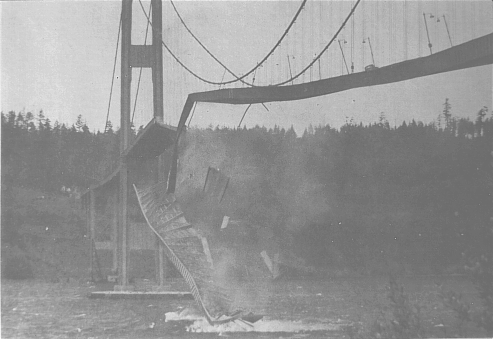
\includegraphics[width=.6\textwidth]{aux/examples/tacoma-narrows-bridge/tacoma-narrows-bridge-collapsed}
\end{figure}
\end{frame}



\begin{frame}
\frametitle{Tacoma Narrows Bridge}
\framesubtitle{Diagnostic}

\begin{itemize}
	\item Due to financing issues, shallower supports-girders 2.4 m deep were
	used.
	\begin{itemize}
		\item This approach meant a slimmer, more elegant design and reduced
		construction costs compared to the original design.
	\end{itemize}

	\item The decision to use shallow and narrow girders proved to be the first
	bridge's undoing.
	\begin{itemize}
		\item With such girders, the roadbed was insufficiently rigid and was
		easily moved about by winds.

		\item Bridge nicknamed as ``Galloping Gertie''.
	\end{itemize}
\end{itemize}
\end{frame}


\begin{frame}
\frametitle{Tacoma Narrows Bridge}
\framesubtitle{Diagnostic}

\begin{itemize}
	\item The failure of the bridge occurred when a never-before-seen twisting
	mode occurred, from winds at a mild 40 miles per hour (64 km/h).

	\item The amplitude of the motion produced by the fluttering increased
	beyond the strength of a vital part, in this case the suspender cables.

	\item Once several cables failed, the weight of the deck transferred to
	the adjacent cables that broke in turn until almost all of the central deck
	fell into the water below the span.
\end{itemize}
\end{frame}



\begin{frame}[hasprev=true, hasnext=false]
\frametitle{Tacoma Narrows Bridge}
\framesubtitle{Solution}

\begin{itemize}
	\item Two solutions were devised:
	\begin{itemize}
		\item Drill some holes in the lateral girders and along the deck so
		that the air flow could circulate through them (in this way reducing
		lift forces).

		\item Give a more aerodynamic shape to the transverse section of the
		deck by adding fairings or deflector vanes along the deck, attached to
		the girder fascia.
	\end{itemize}

	\item The second option was the chosen one; but it was not carried out,
	because the bridge collapsed five days after the solution was proposed.
\end{itemize}
\end{frame}